\documentclass{standalone}
\usepackage{tikz}
\usetikzlibrary{patterns, positioning}
\usepackage[sfdefault]{ClearSans} %% option 'sfdefault' activates Clear Sans as the default text font
\usepackage[T1]{fontenc}

\begin{document}
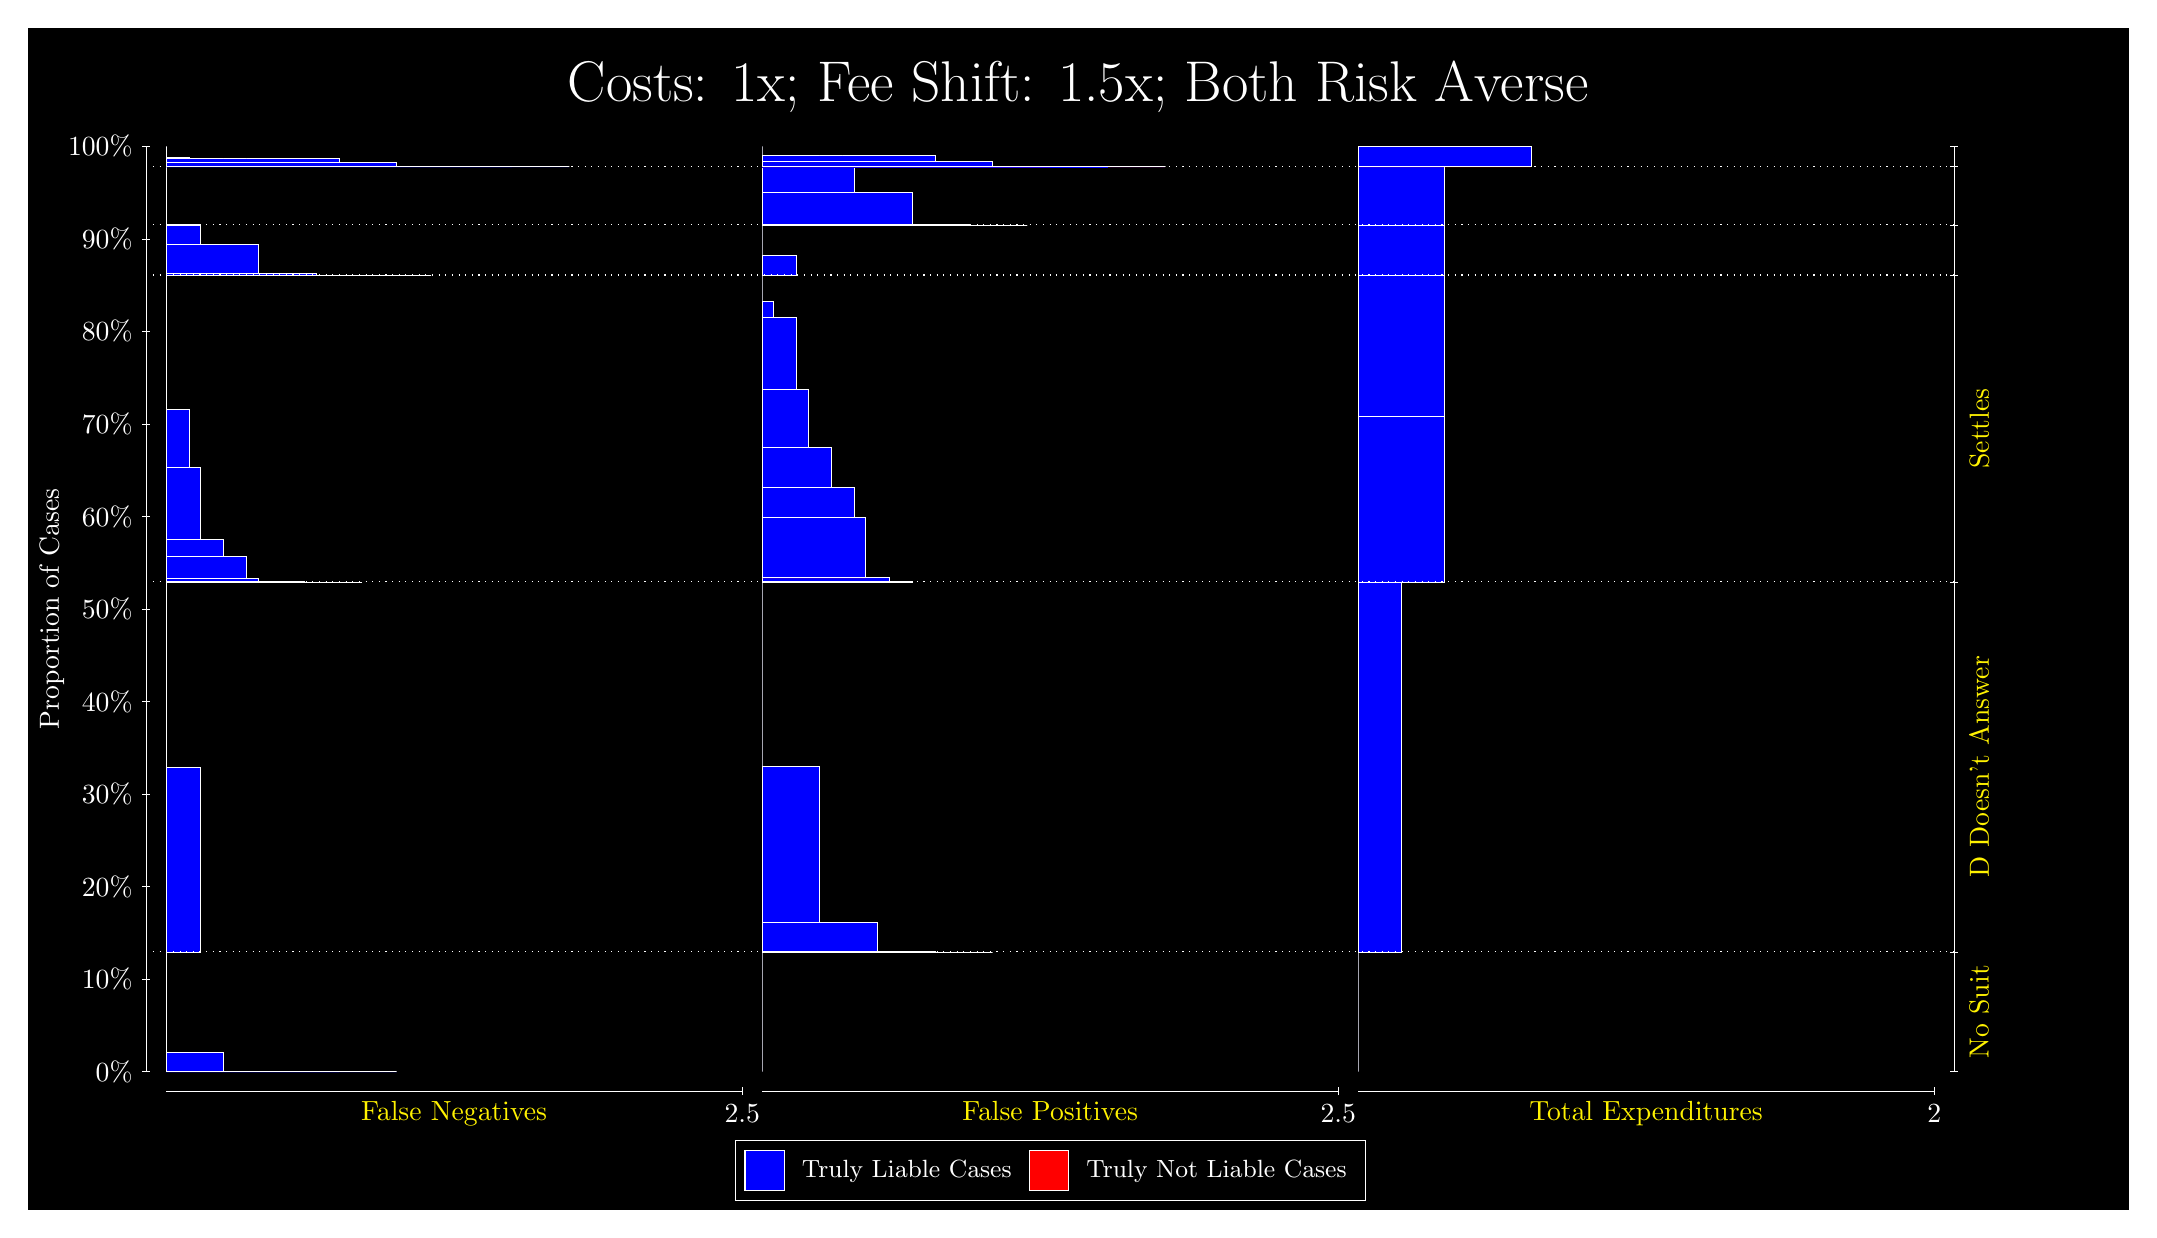
\begin{tikzpicture}
\draw[fill=black] (0,0) rectangle (26.667,15);
\draw[text=white] (0,13.5) rectangle (26.667,15) node[midway] {\huge Costs: 1x; Fee Shift: 1.5x; Both Risk Averse};
\draw[white, very thin] (1.5,1.75) -- (1.5,13.5);
\node[rotate=90, text=white, anchor=center] at (0.3, 7.625) {Proportion of Cases};
\draw[white, very thin] (1.45,1.75) -- (1.55,1.75);
\node[text=white, anchor=east] at (1.45, 1.75) {0\%};
\draw[white, very thin] (1.45,2.925) -- (1.55,2.925);
\node[text=white, anchor=east] at (1.45, 2.925) {10\%};
\draw[white, very thin] (1.45,4.1) -- (1.55,4.1);
\node[text=white, anchor=east] at (1.45, 4.1) {20\%};
\draw[white, very thin] (1.45,5.275) -- (1.55,5.275);
\node[text=white, anchor=east] at (1.45, 5.275) {30\%};
\draw[white, very thin] (1.45,6.45) -- (1.55,6.45);
\node[text=white, anchor=east] at (1.45, 6.45) {40\%};
\draw[white, very thin] (1.45,7.625) -- (1.55,7.625);
\node[text=white, anchor=east] at (1.45, 7.625) {50\%};
\draw[white, very thin] (1.45,8.8) -- (1.55,8.8);
\node[text=white, anchor=east] at (1.45, 8.8) {60\%};
\draw[white, very thin] (1.45,9.975) -- (1.55,9.975);
\node[text=white, anchor=east] at (1.45, 9.975) {70\%};
\draw[white, very thin] (1.45,11.15) -- (1.55,11.15);
\node[text=white, anchor=east] at (1.45, 11.15) {80\%};
\draw[white, very thin] (1.45,12.325) -- (1.55,12.325);
\node[text=white, anchor=east] at (1.45, 12.325) {90\%};
\draw[white, very thin] (1.45,13.5) -- (1.55,13.5);
\node[text=white, anchor=east] at (1.45, 13.5) {100\%};

\draw[white, very thin] (24.457,1.75) -- (24.457,13.5);
\draw[white, very thin] (24.407,1.75) -- (24.507,1.75);
\node[anchor=west] at (24.407, 1.75) {};
\draw[white, very thin] (24.407,3.2701) -- (24.507,3.2701);
\node[anchor=west] at (24.407, 3.2701) {};
\draw[white, very thin] (24.407,7.9683) -- (24.507,7.9683);
\node[anchor=west] at (24.407, 7.9683) {};
\draw[white, very thin] (24.407,11.866) -- (24.507,11.866);
\node[anchor=west] at (24.407, 11.866) {};
\draw[white, very thin] (24.407,12.503) -- (24.507,12.503);
\node[anchor=west] at (24.407, 12.503) {};
\draw[white, very thin] (24.407,13.242) -- (24.507,13.242);
\node[anchor=west] at (24.407, 13.242) {};
\draw[white, very thin] (24.407,13.5) -- (24.507,13.5);
\node[anchor=west] at (24.407, 13.5) {};

\draw[white, very thin, fill=blue] (1.75,1.75) rectangle (4.6775,1.75);
\draw[white, very thin, fill=blue] (1.75,1.75) rectangle (3.9457,1.75);
\draw[white, very thin, fill=blue] (1.75,1.75) rectangle (3.2138,1.7521);
\draw[white, very thin, fill=blue] (1.75,1.7521) rectangle (2.4819,1.9989);
\draw[white, very thin, fill=red] (1.75,1.9989) rectangle (1.75,1.9989);
\draw[white, very thin, fill=blue] (1.75,1.9989) rectangle (1.75,3.2701);
\draw[white, very thin, fill=blue] (1.75,3.2701) rectangle (2.1891,5.6163);
\draw[white, very thin, fill=red] (1.75,5.6163) rectangle (1.75,5.6163);
\draw[white, very thin, fill=blue] (1.75,5.6163) rectangle (1.75,7.9683);
\draw[white, very thin, fill=blue] (1.75,7.9683) rectangle (4.2384,7.9683);
\draw[white, very thin, fill=blue] (1.75,7.9683) rectangle (3.9457,7.9683);
\draw[white, very thin, fill=blue] (1.75,7.9683) rectangle (3.6529,7.9683);
\draw[white, very thin, fill=blue] (1.75,7.9683) rectangle (3.5065,7.9766);
\draw[white, very thin, fill=blue] (1.75,7.9766) rectangle (3.2138,7.9797);
\draw[white, very thin, fill=blue] (1.75,7.9797) rectangle (2.921,8.0193);
\draw[white, very thin, fill=blue] (1.75,8.0193) rectangle (2.7746,8.2993);
\draw[white, very thin, fill=blue] (1.75,8.2993) rectangle (2.4819,8.5055);
\draw[white, very thin, fill=blue] (1.75,8.5055) rectangle (2.1891,9.423);
\draw[white, very thin, fill=blue] (1.75,9.423) rectangle (2.0428,10.156);
\draw[white, very thin, fill=red] (1.75,10.156) rectangle (1.75,10.156);
\draw[white, very thin, fill=blue] (1.75,10.156) rectangle (1.75,11.866);
\draw[white, very thin, fill=blue] (1.75,11.866) rectangle (5.1167,11.866);
\draw[white, very thin, fill=blue] (1.75,11.866) rectangle (4.3848,11.866);
\draw[white, very thin, fill=blue] (1.75,11.866) rectangle (3.6529,11.893);
\draw[white, very thin, fill=blue] (1.75,11.893) rectangle (2.921,12.253);
\draw[white, very thin, fill=blue] (1.75,12.253) rectangle (2.1891,12.503);
\draw[white, very thin, fill=red] (1.75,12.503) rectangle (1.75,12.503);
\draw[white, very thin, fill=blue] (1.75,12.503) rectangle (2.1891,12.507);
\draw[white, very thin, fill=red] (1.75,12.507) rectangle (1.75,12.507);
\draw[white, very thin, fill=blue] (1.75,12.507) rectangle (1.75,13.242);
\draw[white, very thin, fill=blue] (1.75,13.242) rectangle (6.8732,13.242);
\draw[white, very thin, fill=blue] (1.75,13.242) rectangle (6.1413,13.242);
\draw[white, very thin, fill=blue] (1.75,13.242) rectangle (5.4094,13.246);
\draw[white, very thin, fill=blue] (1.75,13.246) rectangle (4.6775,13.299);
\draw[white, very thin, fill=blue] (1.75,13.299) rectangle (3.9457,13.351);
\draw[white, very thin, fill=blue] (1.75,13.351) rectangle (3.5065,13.351);
\draw[white, very thin, fill=blue] (1.75,13.351) rectangle (3.2138,13.352);
\draw[white, very thin, fill=blue] (1.75,13.352) rectangle (2.7746,13.352);
\draw[white, very thin, fill=blue] (1.75,13.352) rectangle (2.7746,13.352);
\draw[white, very thin, fill=blue] (1.75,13.352) rectangle (2.4819,13.352);
\draw[white, very thin, fill=blue] (1.75,13.352) rectangle (2.0428,13.352);
\draw[white, very thin, fill=blue] (1.75,13.352) rectangle (2.0428,13.358);
\draw[white, very thin, fill=red] (1.75,13.358) rectangle (1.75,13.358);
\draw[white, very thin, fill=blue] (1.75,13.358) rectangle (1.75,13.5);
\draw[white, very thin, fill=red] (9.3189,1.75) rectangle (9.3189,1.75);
\draw[white, very thin, fill=blue] (9.3189,1.75) rectangle (9.3189,3.2701);
\draw[white, very thin, fill=red] (9.3189,3.2701) rectangle (12.246,3.2701);
\draw[white, very thin, fill=blue] (9.3189,3.2701) rectangle (12.246,3.2701);
\draw[white, very thin, fill=blue] (9.3189,3.2701) rectangle (11.515,3.273);
\draw[white, very thin, fill=blue] (9.3189,3.273) rectangle (10.783,3.6455);
\draw[white, very thin, fill=blue] (9.3189,3.6455) rectangle (10.051,5.6222);
\draw[white, very thin, fill=blue] (9.3189,5.6222) rectangle (9.3189,7.9683);
\draw[white, very thin, fill=red] (9.3189,7.9683) rectangle (11.222,7.9683);
\draw[white, very thin, fill=blue] (9.3189,7.9683) rectangle (11.222,7.9814);
\draw[white, very thin, fill=red] (9.3189,7.9814) rectangle (10.929,7.9814);
\draw[white, very thin, fill=blue] (9.3189,7.9814) rectangle (10.929,8.0216);
\draw[white, very thin, fill=red] (9.3189,8.0216) rectangle (10.636,8.0216);
\draw[white, very thin, fill=blue] (9.3189,8.0216) rectangle (10.636,8.7946);
\draw[white, very thin, fill=blue] (9.3189,8.7946) rectangle (10.49,9.1729);
\draw[white, very thin, fill=blue] (9.3189,9.1729) rectangle (10.197,9.6777);
\draw[white, very thin, fill=blue] (9.3189,9.6777) rectangle (9.9044,10.411);
\draw[white, very thin, fill=blue] (9.3189,10.411) rectangle (9.758,11.329);
\draw[white, very thin, fill=blue] (9.3189,11.329) rectangle (9.4652,11.535);
\draw[white, very thin, fill=blue] (9.3189,11.535) rectangle (9.3189,11.866);
\draw[white, very thin, fill=red] (9.3189,11.866) rectangle (9.758,11.866);
\draw[white, very thin, fill=blue] (9.3189,11.866) rectangle (9.758,12.116);
\draw[white, very thin, fill=blue] (9.3189,12.116) rectangle (9.3189,12.503);
\draw[white, very thin, fill=red] (9.3189,12.503) rectangle (12.686,12.503);
\draw[white, very thin, fill=blue] (9.3189,12.503) rectangle (12.686,12.503);
\draw[white, very thin, fill=blue] (9.3189,12.503) rectangle (11.954,12.512);
\draw[white, very thin, fill=blue] (9.3189,12.512) rectangle (11.222,12.919);
\draw[white, very thin, fill=blue] (9.3189,12.919) rectangle (10.49,13.239);
\draw[white, very thin, fill=blue] (9.3189,13.239) rectangle (9.758,13.242);
\draw[white, very thin, fill=red] (9.3189,13.242) rectangle (14.442,13.242);
\draw[white, very thin, fill=blue] (9.3189,13.242) rectangle (14.442,13.242);
\draw[white, very thin, fill=red] (9.3189,13.242) rectangle (13.71,13.242);
\draw[white, very thin, fill=blue] (9.3189,13.242) rectangle (13.71,13.243);
\draw[white, very thin, fill=red] (9.3189,13.243) rectangle (12.978,13.243);
\draw[white, very thin, fill=blue] (9.3189,13.243) rectangle (12.978,13.248);
\draw[white, very thin, fill=red] (9.3189,13.248) rectangle (12.246,13.248);
\draw[white, very thin, fill=blue] (9.3189,13.248) rectangle (12.246,13.307);
\draw[white, very thin, fill=blue] (9.3189,13.307) rectangle (11.515,13.384);
\draw[white, very thin, fill=blue] (9.3189,13.384) rectangle (10.783,13.39);
\draw[white, very thin, fill=red] (9.3189,13.39) rectangle (10.344,13.39);
\draw[white, very thin, fill=blue] (9.3189,13.39) rectangle (10.344,13.39);
\draw[white, very thin, fill=blue] (9.3189,13.39) rectangle (10.051,13.39);
\draw[white, very thin, fill=red] (9.3189,13.39) rectangle (9.6116,13.39);
\draw[white, very thin, fill=blue] (9.3189,13.39) rectangle (9.6116,13.392);
\draw[white, very thin, fill=red] (9.3189,13.392) rectangle (9.3189,13.392);
\draw[white, very thin, fill=blue] (9.3189,13.392) rectangle (9.3189,13.5);
\draw[white, very thin, fill=red] (16.888,1.75) rectangle (16.888,1.75);
\draw[white, very thin, fill=blue] (16.888,1.75) rectangle (16.888,3.2701);
\draw[white, very thin, fill=red] (16.888,3.2701) rectangle (17.437,3.2701);
\draw[white, very thin, fill=blue] (16.888,3.2701) rectangle (17.437,7.9683);
\draw[white, very thin, fill=red] (16.888,7.9683) rectangle (17.986,7.9683);
\draw[white, very thin, fill=blue] (16.888,7.9683) rectangle (17.986,10.071);
\draw[white, very thin, fill=red] (16.888,10.071) rectangle (17.986,10.071);
\draw[white, very thin, fill=blue] (16.888,10.071) rectangle (17.986,11.866);
\draw[white, very thin, fill=red] (16.888,11.866) rectangle (17.986,11.866);
\draw[white, very thin, fill=blue] (16.888,11.866) rectangle (17.986,12.503);
\draw[white, very thin, fill=red] (16.888,12.503) rectangle (17.986,12.503);
\draw[white, very thin, fill=blue] (16.888,12.503) rectangle (17.986,13.242);
\draw[white, very thin, fill=red] (16.888,13.242) rectangle (19.083,13.242);
\draw[white, very thin, fill=blue] (16.888,13.242) rectangle (19.083,13.5);
\draw[white, dotted] (1.5,3.2701) -- (24.457,3.2701);
\draw[white, dotted] (1.5,7.9683) -- (24.457,7.9683);
\draw[white, dotted] (1.5,11.866) -- (24.457,11.866);
\draw[white, dotted] (1.5,12.503) -- (24.457,12.503);
\draw[white, dotted] (1.5,13.242) -- (24.457,13.242);
\draw[white, very thin] (1.75,1.5) -- (9.0689,1.5);
\node[text=yellow, anchor=north] at (5.4094, 1.5) {False Negatives};
\draw[white, very thin] (9.0689,1.45) -- (9.0689,1.55);
\node[text=white, anchor=north] at (9.0689, 1.45) {2.5};

\draw[white, very thin] (9.3189,1.5) -- (16.638,1.5);
\node[text=yellow, anchor=north] at (12.978, 1.5) {False Positives};
\draw[white, very thin] (16.638,1.45) -- (16.638,1.55);
\node[text=white, anchor=north] at (16.638, 1.45) {2.5};

\draw[white, very thin] (16.888,1.5) -- (24.207,1.5);
\node[text=yellow, anchor=north] at (20.547, 1.5) {Total Expenditures};
\draw[white, very thin] (24.207,1.45) -- (24.207,1.55);
\node[text=white, anchor=north] at (24.207, 1.45) {2};

\node[text=yellow, centered, rotate=90] at (24.777, 2.5101) {No Suit};
\node[text=yellow, centered, rotate=90] at (24.777, 5.6192) {D Doesn't Answer};
\node[text=yellow, centered, rotate=90] at (24.777, 9.917) {Settles};




\draw (12.978300999999998,1.5) node[draw=none] (baseCoordinate) {};
\begin{scope}[align=center]
        \matrix[scale=0.5, draw=white, below=0.5cm of baseCoordinate, nodes={draw}, column sep=0.1cm]{
            \node[rectangle, draw, minimum width=0.5cm, minimum height=0.5cm, fill=blue] {}; &
            \node[draw=none, font=\small, text=white] (B) {Truly Liable Cases}; &
            \node[rectangle, draw, minimum width=0.5cm, minimum height=0.5cm, fill=red] {}; &
            \node[draw=none, font=\small, text=white] (B) {Truly Not Liable Cases}; \\
            };
\end{scope}

\end{tikzpicture}
\end{document}